%!TEX TS-program = xelatex
\documentclass[]{friggeri-cv}
\usepackage{afterpage}
\usepackage{hyperref}
\usepackage{color}
\usepackage{xcolor}
\hypersetup{
    pdftitle={},
    pdfauthor={},
    pdfsubject={},
    pdfkeywords={},
    colorlinks=false,       % no lik border color
   allbordercolors=white    % white border color for all
}
\addbibresource{bibliography.bib}
\RequirePackage{xcolor}
\definecolor{pblue}{HTML}{0395DE}

\begin{document}
\header{Ibrahim}{Essam}
      {Mechatronics Engineer}
      
% Fake text to add separator      
\fcolorbox{white}{gray}{\parbox{\dimexpr\textwidth-2\fboxsep-2\fboxrule}{%
.....
}}

% In the aside, each new line forces a line break
\begin{aside}
 \textcolor{lightgray}{                    }
    Male,19.07.1995
    Egyptian
  \section{Address}
    El-Rehab
    11841, New Cairo, Egypt
    ~
  \section{Telephone}
    +201110731015
    ~
  \section{Mail}
    \href{mailto:ibrahim.essam1995@gmail.com}{ibrahim.essam1995@\\gmail.com}
    ~
  \section{LinkedIn}
    ~  
   
\includegraphics[scale=0.20]{img/qr.jpg}
    ~
  \section{Programming}
    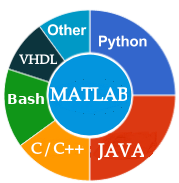
\includegraphics[scale=0.62]{img/programming.png}
    ~
  \section{Programs}
    \textbf{MATLAB}
\includegraphics[scale=0.40]{img/5stars.png}
    \textbf{20Sim}
\includegraphics[scale=0.40]{img/3stars.png}
    \textbf{LabView}
\includegraphics[scale=0.40]{img/3stars.png}
    \textbf{Solidworks}
\includegraphics[scale=0.40]{img/2stars.png}
    \textbf{CANoe}
\includegraphics[scale=0.40]{img/1stars.png}
    ~
  \section{Personal Skills}
    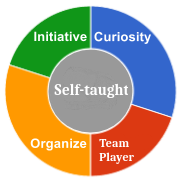
\includegraphics[scale=0.62]{img/personal.png}
    \textcolor{orange}{{\small Link}}  
\includegraphics[scale=0.1]{img/orange.png}
\end{aside}
A fresh graduate Mechatronics engineer searching for a challenging long-term internship in the Industry where I can apply my knowledge and gain practical experience.  
\section{Education}
\begin{entrylist}
 \entry
    {02/17 - 08/17}
    {Bachelor Thesis Project}
    {Daimler AG (Mercedes-Benz R\&D)}
    {Title:"Front- and Backened Development of a Test Robot for Touch Devices"\\
    Grade: \textbf{B+} 
    
    }
  \entry
    {2013 - 2018}
    {Bachelor Degree in Mechatronics Engineering}
    {The German University in Cairo}
    {GPA 1.37 Equivalent To \textbf{Excellent with Honours}\\
   }
    
     \entry
    {2010 - 2013}
    {Egyptian Thanwya Amma - High School}
    {Al-Minofya, Egypt}
    {Top ranked student with 99.7 \% score.\\
    }
  \end{entrylist}
\section{Experience}
\begin{entrylist}
  \entry
    {02/17 - 08/17}
    {Daimler AG (Mercedes-Benz RD/UKC)}
    {Sindelfingen, Germany}
    {3 Months Internship followed by 3 Months bachelor thesis.I was responsible of the following tasks.
    \begin{itemize}
        \item Hardware (Robot Construction,Kinematics and Touch Devices)
        \item Software (CANoe,CAN-bus,Databases and The Test System)
        
        \item Making Tests on The Touch Devices with the Robot to analyze the state and develop improvements.
        \item Implementing new Algorithms and Data structures for the Robot in MATLAB.
        \item Programming a Graphical User Interface for the System
        \item Optimizing the test system to fulfill the requirements of Daimler AG.
    \end{itemize}}
  \entry
    {03/16 - 02/17}
    {GUC Innovators - Shell Eco Marathon Competition}
    {Cairo,Egypt}
    {Design and Manufacturing of Car's Steering and Chassis }
    \entry
    {06/16 - 07/16}
    {EgyptAir Summer Training}
    {Cairo Airport,Egypt}
    {EgyptAir Maintenance \& Engineering training programs.}
    \entry
    {07/16 - 08/16}
    {GlaxoSmithKline Summer Internship}
    {El-Salam City, Egypt}
    {Summer Internship in GSK at the Production Department.}
    \entry
    {10/14 - 02/15}
    {Junior Teaching Assistant}
    {The German University in Cairo}
    {Teaching CS01 Students Programming Concepts and Assisting them during the Labs}
\end{entrylist}
\section{Honors \& Awards}
\begin{entrylist}
  \entry
    {09/2013}
    {\href{https://drive.google.com/open?id=19nxGmnJJkMHri0zitiv5pXWpjLnGhKvk}{ \textcolor{orange}{Academic Achievement Full Scholarship}}}
    {The German University in Cairo}
    {\emph{}}
    \entry
    {07/2013}
    {Top Ranked Student With 99.7 \% Score}
    {The Ministry of Education}
    {\emph{}}
   \end{entrylist}
   \section{Extracurricular activities}
   \begin{itemize}
   \item  Y.E.S (Youth Establishing Skills) Team Member at Bdaya.
 
   \end{itemize}
\section{Online Courses \& Certificates}
\begin{entrylist}
\entry
    {07/2018}
    {\href{https://www.coursera.org/verify/specialization/PLESFRLGX57Y}{\textcolor{orange}{Machine Learning with TF on GCP Specialization }} }
    { Google Cloud }
    {\emph{}}
\entry
    {07/2018}
    {\href{https://www.coursera.org/account/accomplishments/specialization/certificate/X8GDFN8YHAU6}{\textcolor{orange}{Deep Learning, a 5-course specialization}} }
    { deeplearning.ai }
    {\emph{}}
 \entry
    {03/2018}
    {\href{https://courses.edx.org/certificates/3d94e47ded1e49649d358c7d8fd12989}{\textcolor{orange}{Electric and Conventional Vehicles}} }
    { Chalmers University of Technology }
    {\emph{}}
   \entry
    {03/2018}
    {\href{https://www.coursera.org/account/accomplishments/certificate/3V9G5VAVE93F}{\textcolor{orange}{Agile Software Development}} }
    {University of Minnesota}
    {\emph{}}
  \entry
    {01/2018}
    {\href{https://www.coursera.org/account/accomplishments/certificate/G5QLQYHBYCJR}{\textcolor{orange}{FPGA Design for Embedded Systems}} }
    {CU Boulder}
    {\emph{}}
  \entry
    {11/2017}
    {\href{https://www.coursera.org/account/accomplishments/verify/U4HKE8MNY33F}{\textcolor{orange}{Embedded Systems Software and Devel. Environments} }}
    {CU Boulder}
    {\emph{}}
    \entry
    {08/2017}
    {\href{https://www.coursera.org/account/accomplishments/verify/J6YH5LSNL4CF}{\textcolor{orange}{Control of Mobile Robots on Coursera}} }
    {Georgia Institute of Technology}
    {\emph{}}
  
   \end{entrylist}
   \begin{aside}
   \section{GitHub}
github.com/HemaZ   
~
\section{Languages}
    \textbf{Arabic}
\includegraphics[scale=0.40]{img/5stars.png}
    \textbf{English}
\includegraphics[scale=0.40]{img/4stars.png}
    \textbf{German}
\includegraphics[scale=0.40]{img/3stars.png}
    ~
    \section{OS Preference}
    {\small \textbf{Ubuntu/Linux}}
\includegraphics[scale=0.40]{img/5stars.png}
    \textbf{Windows}
\includegraphics[scale=0.40]{img/4stars.png}
    \textbf{MacOS}
\includegraphics[scale=0.40]{img/1stars.png}
    ~
        \section{Frameworks}
	~        
     
\includegraphics[scale=0.13]{img/pt.png}
     
\includegraphics[scale=0.04]{img/tf.png}
     
\includegraphics[scale=0.18]{img/K.jpg}
     
\includegraphics[scale=0.1]{img/ros2.png}
     
\includegraphics[scale=0.3]{img/Untitled.png} \\     OpenCV Library     
    ~
     \section{MCUs}
     \textbf{Atmel AVR}
\includegraphics[scale=0.40]{img/4stars.png}
     \textbf{PIC16F}
\includegraphics[scale=0.40]{img/3stars.png}
    ~
         \section{Controllers}
     \textbf{PID}
\includegraphics[scale=0.40]{img/5stars.png}
     \textbf{\small LQR/LQG}
\includegraphics[scale=0.40]{img/5stars.png}
       \textbf{\small MPC}
\includegraphics[scale=0.40]{img/5stars.png}
              \textbf{\small Nonlinear}
\includegraphics[scale=0.40]{img/4stars.png}
\textbf{\small Adaptive}
\includegraphics[scale=0.40]{img/3stars.png}
                                   \textbf{\small Robust}
\includegraphics[scale=0.40]{img/3stars.png}
    ~
   \end{aside}
\section{Projects}
\begin{entrylist}
 \entry
    {2018}
    {Cars Detection using YOLOV2 Algorithm}
    {-}
    {YOLO V2 Trained on COCO Dataset and Darkent Weights for cars detection\\
    {\href{https://www.youtube.com/watch?v=NPndZq2cXKE}{\textcolor{orange}{https://www.youtube.com/watch?v=NPndZq2cXKE}} }}
  \entry
    {2018}
    {Images Recognition and Translation (DeepLearning)}
    {-}
    {Qt5 Python Application to Load image from a URL, Recognises the object and Translate it into German.
    Using ResNet50 trained on imagenet . \\
    {\href{https://github.com/HemaZ/imgRecgTrans}{\textcolor{orange}{https://github.com/HemaZ/imgRecgTrans}} }}
  \entry
    {2018}
    {Autonomous Mobile Robot (Turtle Bot)}
    {The German University in Cairo}
    {Autonomus Mobile Robot, which navigates and creates a map of the environment. using Odometry sensors and communicating via ROS(Robotics Operating System) network to simulate the Tasks. \\
    {\href{https://www.youtube.com/watch?v=ThAjbMSuvAo}{\textcolor{orange}{https://www.youtube.com/watch?v=ThAjbMSuvAo}} }}
     \entry
    {2018}
    {Optimal Control of Wind Turbine}
    {The German University in Cairo}
    {Designing and Simulating an Optimal LQG Control For Wind turbines using Kalman Filter  .
    }
    \entry
    {2018}
    {2D Plotter Robot Arm}
    {The German University in Cairo}
    {2-DOF SCARA plotter Robot Arm with Computed Torque Controller. The Design was made on Solidworks then manufactured and assembled.We Used Nonlinear Controller instead of the regular PD controller.  .
    }
           \entry
    {2018}
    {Cars Plates Detection (Image Processing)}
    {The German University in Cairo}
    {Applying some of The Image Processing Algorithms on Matlab to Detect Cars Plates.\\
    https://www.youtube.com/watch?v=PQmAcP1iBfw  .
    }
           \entry
    {2016}
    {Self-Balancing Two Wheeled Robot}
    {The German University in Cairo}
    {Segway Or Inverted Pendulum Control using PID controller and Kalman Filter for The IMU Readings.\\
    https://www.youtube.com/watch?v=lp5exim\textunderscore Jro  .
    }
          
               \entry
    {2016}
    {Yu-Gi-Oh Video Game Using Java}
    {The German University in Cairo}
    {CS4 Final Project. The Game was choosed as one of the top 14 project this year.\\
    https://www.youtube.com/watch?v=wY9EOFwh1F0m\textunderscore Jro  .
    }    
                      
  \end{entrylist}   
\end{document}
